% !TEX encoding = UTF-8 Unicode
% !TEX program = pdflatex
% !TEX spellcheck = en_US


% In order to correctly compile this document,
% execute the following commands:
% 1. pdflatex
% 2. pdflatex
% 3. pdflatex



\documentclass[amsthm,ebook]{saparticle}

% IF YOU USE PDFLATEX
\usepackage[utf8x]{inputenc}
% if you write in english and in greek
\usepackage{ucs}
\usepackage[greek,english]{babel}
\languageattribute{greek}{polutoniko}

% IF YOU USE XELATEX
%\usepackage{polyglossia}
% if you write in italian
%\setmainlanguage{italian}
% If you want put some ancient greek:
%\setotherlanguage[variant=polytonic]{greek}
%\newfontfamily{\greekfont}[Ligatures=TeX]{Palatino Linotype}

% dummy text (remove in a normal thesis)
% remove if not necessary
\usepackage{siunitx}
%Natbib for bibliography management
\usepackage[authoryear]{natbib}
% custom commands
\newcommand{\bs}{\textbackslash}

%%%%%%%%
%TITLE:%
%%%%%%%%
\title{Infrastructures for Digital Research: New opportunities and challenges}
\author[gla]{Lorna Hughes\corref{first}}
\address[uniba]{Humanities Advanced Technology and Information Institute. University of Glasgow} 
\cortext[first]{Corresponding author. Email: Lorna.Hughes@glasgow.ac.uk}

\begin{document}
\maketitle
\begin{abstract}
This article is based on a keynote presentation given at the EAGLE Conference, Sapeinza University, Rome, on January 29th 2016. It draws on the author’s experience in digital humanities and in developing a digital collections research programme based in the National Library of Wales as an evidence base for understanding ways that the use and impact of digital cultural heritage can be enhanced and increased: an understanding that can provide a critical framework for future development of digital content by Galleries, Libraries, Archives and Museums (the so-called GLAM) sector.  This research is currently informing approaches to developing and using digital content in research that will be delivered through Europeana Research, a programme of engagement with the research community to make the metadata and content of Europeana.eu more accessible for research. This programme will have wider applicability for the development of other Research Infrastructures in the Arts and Humanities, cultivating a better awareness of the conditions that encourage use and re-use of digital heritage for research, ultimately enabling further exploitation of the ‘digital turn’ through the use of content, methods and content for research.
\end{abstract}

\section{Introduction: understanding the use of digital content}

The past twenty years has seen a very visible expansion of the digitization of Europe’s Cultural Heritage. However, to put the scale of this investment in perspective, the ENUMERATE\footnote{\url{http://www.enumerate.eu/}} project has produced data about the volume of digital cultural heritage available across Europe. The results of their analysis published in 2014 \cite[6]{ENUMERATE:2014aa} shows that over 10\% of the collections of European museums, archives and libraries has been digitized, over 300 million items. At the present scale of progress, it will take over 30 years to digitize the rest: a task that will be more complex taking into consideration that a large amount of material remaining to be digitized is 20th and 21st century material, either moving image, audio, or born-digital. A growing number of organisations have developed digital strategies to address this: 36\% of the institutions surveyed by ENUMERATE in 2014 have a written digitisation strategy. 


Of the content that has been digitized, though, only 34\% is available online, and of that only 3\% is available for open re-use, though Creative Commons and unrestricted licensing. However, more than half of the organisations surveyed do not implement measures to quantify how their digital content is used. This lack of analysis of use isn’t just an issue in cultural heritage digitization: in 2008, the UK’s Arts and Humanities Research Council carried out an analysis of sustainability planning for projects funded through its Resource Enhancement Scheme, 173 projects, an investment of approximately £40 million \citep{Robey:2008aa}. Of these projects, only just over half were collecting usage statistics \citep[153]{Robey:2011aa}. A lack of enquiry into the use and impact of digital content is not a new issue: indeed, there has been a disproportionate investment in creation, management and curation of digital resources versus use of digital content for scholarship (in the UK from 1999-2009, the AHRC invested approximately £1.5 million into research that addressed the use of digital content, tools, and methods for research, but during this period they invested significantly more in digital content creation and curation). The lack of investigation in this area raises some serious questions about the value of the significant international investment in digital cultural heritage.
 
\section{What are we doing with all this digital stuff?}

It is perplexing that more institutions don’t try to develop a better understanding of what their users do with digital content, because methodologies exist for gathering and analyzing this information. Using analytic tools including Google Analytics\footnote{\url{https://www.google.co.uk/analytics/}} as a baseline, it is possible to augment numeric data with other qualitative and quantitative measures fro assessing users, including structured surveys, interviews, and content analysis tools (looking at citations of digital content, and its embedding in blogs and other resources). These approaches have been refined in a tried and tested approach developed by the Oxford Internet Institute (OII), called Tools for the Impact of Digitised Scholarly Resources (TIDSR)\footnote{\url{http://microsites.oii.ox.ac.uk/tidsr/}}. This has been used successfully to measure the impact of a range of resources in the arts and humanities\footnote{For an overview of the use of this method on a collection of Northeren Irish Parlaimentary Papers, see \citet{Hughes:2015aa}.}.  Similarly, methods developed by the CIBER initiative\footnote{\url{http://ciber-research.eu/}}, originally based at University College London, enable an understanding of the `digital footprint' of users of heritage content\footnote{\url{https://www.ucl.ac.uk/news/news-articles/1001/10010802}, and see also \citet{Nicholas:2014aa}.}. These approaches are an interesting way to build a narrative around data: using statistics about use to build a picture of engagement with digital cultural heritage. Overall a striking finding is the change in information seeking behaviours: users will multitask, and do many things lightly rather than one thing deeply: they have become what David Nicholas of CIBER referred to as `web foxes' \citep{Nicholas:2015aa} as people bounce around the digital domain using fast and abbreviated searches. Visitors to sites will frequently only access one page, then move on. This is even more noticeable when users access heritage data using mobile phones devices on the go: searching is shorter, and less engaged. 

In order to investigate these questions in more detail, from 2011-14 I undertook some analysis of the use of the collections of the National Library of Wales, specifically \emph{Welsh Journals Online} and \emph{Rhyfel Byd 1914-1918 a’r profiad Cymreig / Welsh experience of the First World War 1914-1918}\footnote{\emph{Welsh Journals Online}: \url{http://welshjournals.llgc.org.uk/}; \emph{Cymru 1914-1918a}: \url{http://www.cymru1914.org}. The study into the use of Welsh Journals Online was written about in \citet{Hughes:2012aa}; the research into the use of Cymru1914.org was presented at the Sheffield Digital Humanities Conference, 2014: \url{http://www.hrionline.ac.uk/dhc/paper/19}}. This analysis showed several interesting things. Google analytic data for both sites showed that users mostly come from search engines, not the library website or interface, which is interesting in terms of the investment in presenting content. Similarly, many users were referred through family history websites, or media stories about the resource, rather than academic or subject-specific resources that linked to it: the highest number of referrals to \emph{Rhyfel Byd 1914-1918 a’r profiad Cymreig / Welsh experience of the First World War 1914-1918} came from a story on the BBC Wales News Website about the launch of the resource\footnote{\url{http://www.bbc.co.uk/news/uk-wales-25126781}}. The most popular search results are location based: people are looking for historic information about places they know. Interviews with selected groups of users of both resources expanded on these findings, establishing that the search box enabled most searches: that the `googlization' of information seeking had not affected the quality of information they were able to find. In fact, the only limitation that users reported was that there was not enough digital content in each resource. This is a consistent finding when surveying users of digital cultural heritage: as fast as digital content is launched, the demand increases for more material: `we have too many digital collections' said no survey respondent, ever. The benefits of unlimited access to information are so great that they compensate for problems that arise from irrelevant data, poor metadata, or digital dead ends. 

\section{`We are all digital humanists now'}

Humanities research also exemplifies this enthusiastic embrace of the digital: In many respects, we are all digital humanists now:  we all use digital data for research by default (at the very least, electronic catalogues that point to analogue resources). Scholars rely on a steady consumption of digital source materials for scholarship and pedagogy, mostly created through large-scale digitisation initiatives in universities, libraries, museums and archives and as well as by commercial entities \citep{Ell:2013aa}. And humanists do not just use data: many scholars now create and manage these resources; we communicate via blogs and twitter, and use digital dissemination methods for sharing and challenging research results.  For many, this represents a sea change in research practice within the recognizable lifetime of a career.

But digital humanities is more than just the use of digital content for searching and browsing. If I was to attempt a definition of \emph{`digital humanities'} as an emerging field of research, I would suggest that it is combination of using digital content; with digital methods for the analysis and interpretation of this content; tools for specific scholarly tasks; and communicating research to the widest possible audience using traditional and non-traditional publishing methods. At its most effective, digitally enabled research in the humanities can facilitate and enhance existing research, making research processes easier via the use of computational tools and methods. More interestingly, it can enable research that would be impossible to undertake without digital resources and methods, allowing the formulation of new research questions that are driven by insights only achievable through the use of new tools and methods.

At the core of this sort of approach is collaboration: with researchers from scientific and other humanities disciplines, computational and technical fields, as well as cultural heritage organizations. Another important collaboration is with the audiences for our work, as user-led design, and participation via mechanisms like crowdsourcing, informs the development of many initiatives. It also relies on underlying technical infrastructures.

I like this characterization of digital humanities as about \emph{content, tools and methods}, because it creates a working environment with raw materials, tools for working with the raw material, and expertise in digital methods. This may seem a reduction of humanities practice, one that confirms Gary Hall’s view of the digital humanities as a use of tools and technologies that does not rely on a theoretical framework \citep{Hall:2012aa}: the sort of model that one can see as the basis for a DH research infrastructure, putting the maker’s perspective at the centre.  However, another school of thought in the digital humanities, exemplified by Alan \citet{Liu:2012aa}, sees the emphasis on building and making as a space for exploring and critique of culture. I would argue that the maker and theorist perspectives are not incompatible: in fact, it is through developing and building digital projects in the humanities \emph{through practice} that we can conduct cultural and critical analysis, by questioning many of the assumptions on which digital resources are built and communicated, and developing a better framework for understanding the ways that working with digital content, tools and methods is transforming our consumption and production of knowledge. By subsequently analyzing use of the digital collections and content that have been built, we can also develop a better understanding of their role in the humanities research lifecycle, and start to address questions about how digital content in particular is not just helping us to do research more effectively, but a disruptive, transformative intervention in the research lifecycle. 

To address some of these questions, from 2011-15 the European Science Foundation funded the Research Network in Digital Methods in the Arts and Humanities (NeDiMAH.eu), to look at the practice of digital humanities across Europe, and to understand what researchers need in order to do digitally enabled research in the future. From a detailed programme of methodologically focused activities, several conclusions can be drawn about what can make digital resources and collections more valuable for scholarship\footnote{Full reports of all NeDiMAH activities are available at the Network’s website, \url{nedimah.eu}. These activities were structured around Working Groups, each addressing a specific area of Digital Humanities methods: Space and Time; Information Visualization; Linked Data and Ontological Methods; Developing Digital Data; Large-Scale Text Collections; and Scholarly Digital Editions.}. These conclusions sit alongside the user analysis described above to suggest three core observations about what the research community needs from digital content, and the infrastructures that deliver this content: access to, and `knowability' of digital content; opening up content for use and re-use; and creating better environments for drawing together multimedia content from a variety of sources for analysis and publication. These are described in more detail in the sections that follow. 

\section{Access to, and `knowability' of digital content}

Much of what is classified as `digital humanities' is consumption: scholarly use of digital resources and born-digital material, working in what Roy \citet[22]{Rosenzweig:2010aa} called a culture of abundance.

 While this presents new possibilities it also raises significant challenges, and there is a need for a deeper understanding of the digital resources scholars rely on. As Tim \citet{Hitchcock:2013aa} has described in his article \emph{`confronting the digital: or how academic history writing lost the plot'}, researchers often work with data that is what we would charitably call ‘limited’ in its potential for re-use, thanks to problems with OCR, markup, and description and provenance information. Similarly, limitations in metadata often mean that while keyword searching gives the satisfying `quick hit' of a result, the user frequently misses important contextual information that enables more mindful engagement with sources, especially archival content: the scale of the original sources, their condition and their environment are often hidden when using digital surrogates that often appear as disembodied objects, separated from their context. Ryan \citet{Cordell:2015aa}, who has theorized a `network-author' function in antebellum newspapers from research based on digital newspaper archives, has said that `most digital archives hide more than they reveal, as keyword searches require prior knowledge of the texts to be discovered and can lead to evidentiary excess'.

Another issue is the selection of content for digitization. Due to limitations of funding, availability of analogue sources, and copyright and licensing issues, many digital archives are not ‘complete’. The National Library of Wales received funding from the Welsh Government and European Regional Development Fund (ERDF) to digitize 1 million pages of \emph{Welsh Newspapers Online}\footnote{\url{http://newspapers.library.wales/}} from its holdings. These date from 1800-1919, in Welsh and English. As a selection of the newspaper coverage of the time, this is an important resource for research and teaching: however, it is by no means a full representation of all newspapers of the period. 

%<Figure 1 Home page: Welsh Newspapers Online>
\begin{figure}[!htbp]
\centering
 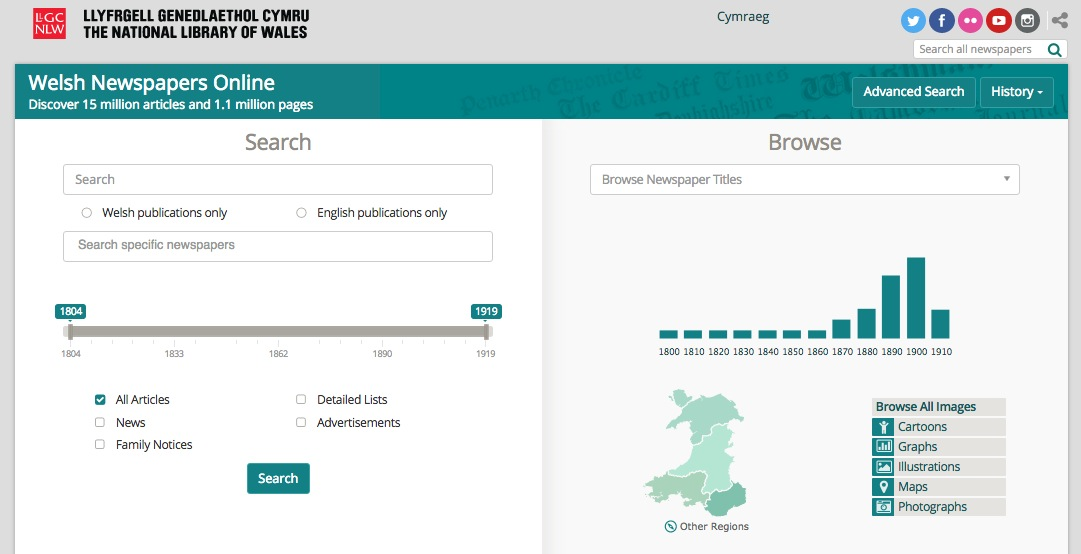
\includegraphics[scale=.28]{img/fig1.jpg}
\caption{Home page: Welsh Newspapers Online}
\label{fig:1}
\end{figure}

Figure \ref{fig:1} shows a chart on the home page of the resource showing the materials selected for digitization: many are missing from the 1909-19 period as a smaller, separate funding source was used for this. From the earlier period, many of the newspaper runs held by the library are incomplete. However, for the user, it’s too easy to assume that the resource is a complete representation of \emph{all} Welsh Newspapers, ever: the chart only shows the proportion of the newspapers in the resource, not as a proportion of those published. As we know, users (especially students) frequently turn to digital content by default when looking for historical sources, and as a free resource, this newspaper archive is very likely to be used, leading to the likelihood of research being conducted from an incomplete dataset. 

\section{Opening up content for use and re-use}

A second requirement for researchers is the need for better, and more open, solutions for analysis and linking of digital content, which is all too frequently locked in digital silos, unable to be easily re-used and linked with other data from other providers and collections. Evaluation of users of digital content, and assessment of a range of European Digital Humanities projects, shows that scholars frequently have very simple questions or ideas that they want to test with data at the desktop, and they do not want the technology to be a barrier. When data is locked in ‘silos’, it can be difficult for the end user to integrate the tools they need analysis and linking with content held remotely. There needs to be greater disassociation of text and data from platform and delivery mechanisms, liberating digital resources for purposes unanticipated by the creators of digital resources \citep{Robinson:2014aa}. 

For example, users often want to be able to use simple, pattern-finding tools, like nGram, with a range of data sets to quickly test hypotheses – the example in Figure 2 shows a visualization, using nGram, of the term `Belgian Refugees' in newspapers in Welsh Newspapers Online from 1914-1919. The graph shows a spike of heightened interest in the almost fashionable cause of Belgian refugees in late 1914, which tailed off as the war continued. A similar pattern can be seen in newspapers from around the British Isles\footnote{\citet{Hughes:2016aa}. The data for this graph is accessible at \url{http://dx.doi.org/10.5525/gla.researchdata.301}}. For questions like this, requiring simple pattern finding, this sort of tool can be a compelling and timesaving aid for researchers. However, as the tool is not part of the resource, using it with this collection required liaison with the National Library of Wales developer team to extract and work with the core data in this way.

One of the huge advantages of digital access is making the invisible visible in archives. We lose this when we can’t easily re-use and re-purpose this content. 

\begin{figure}[!htbp]
\centering
 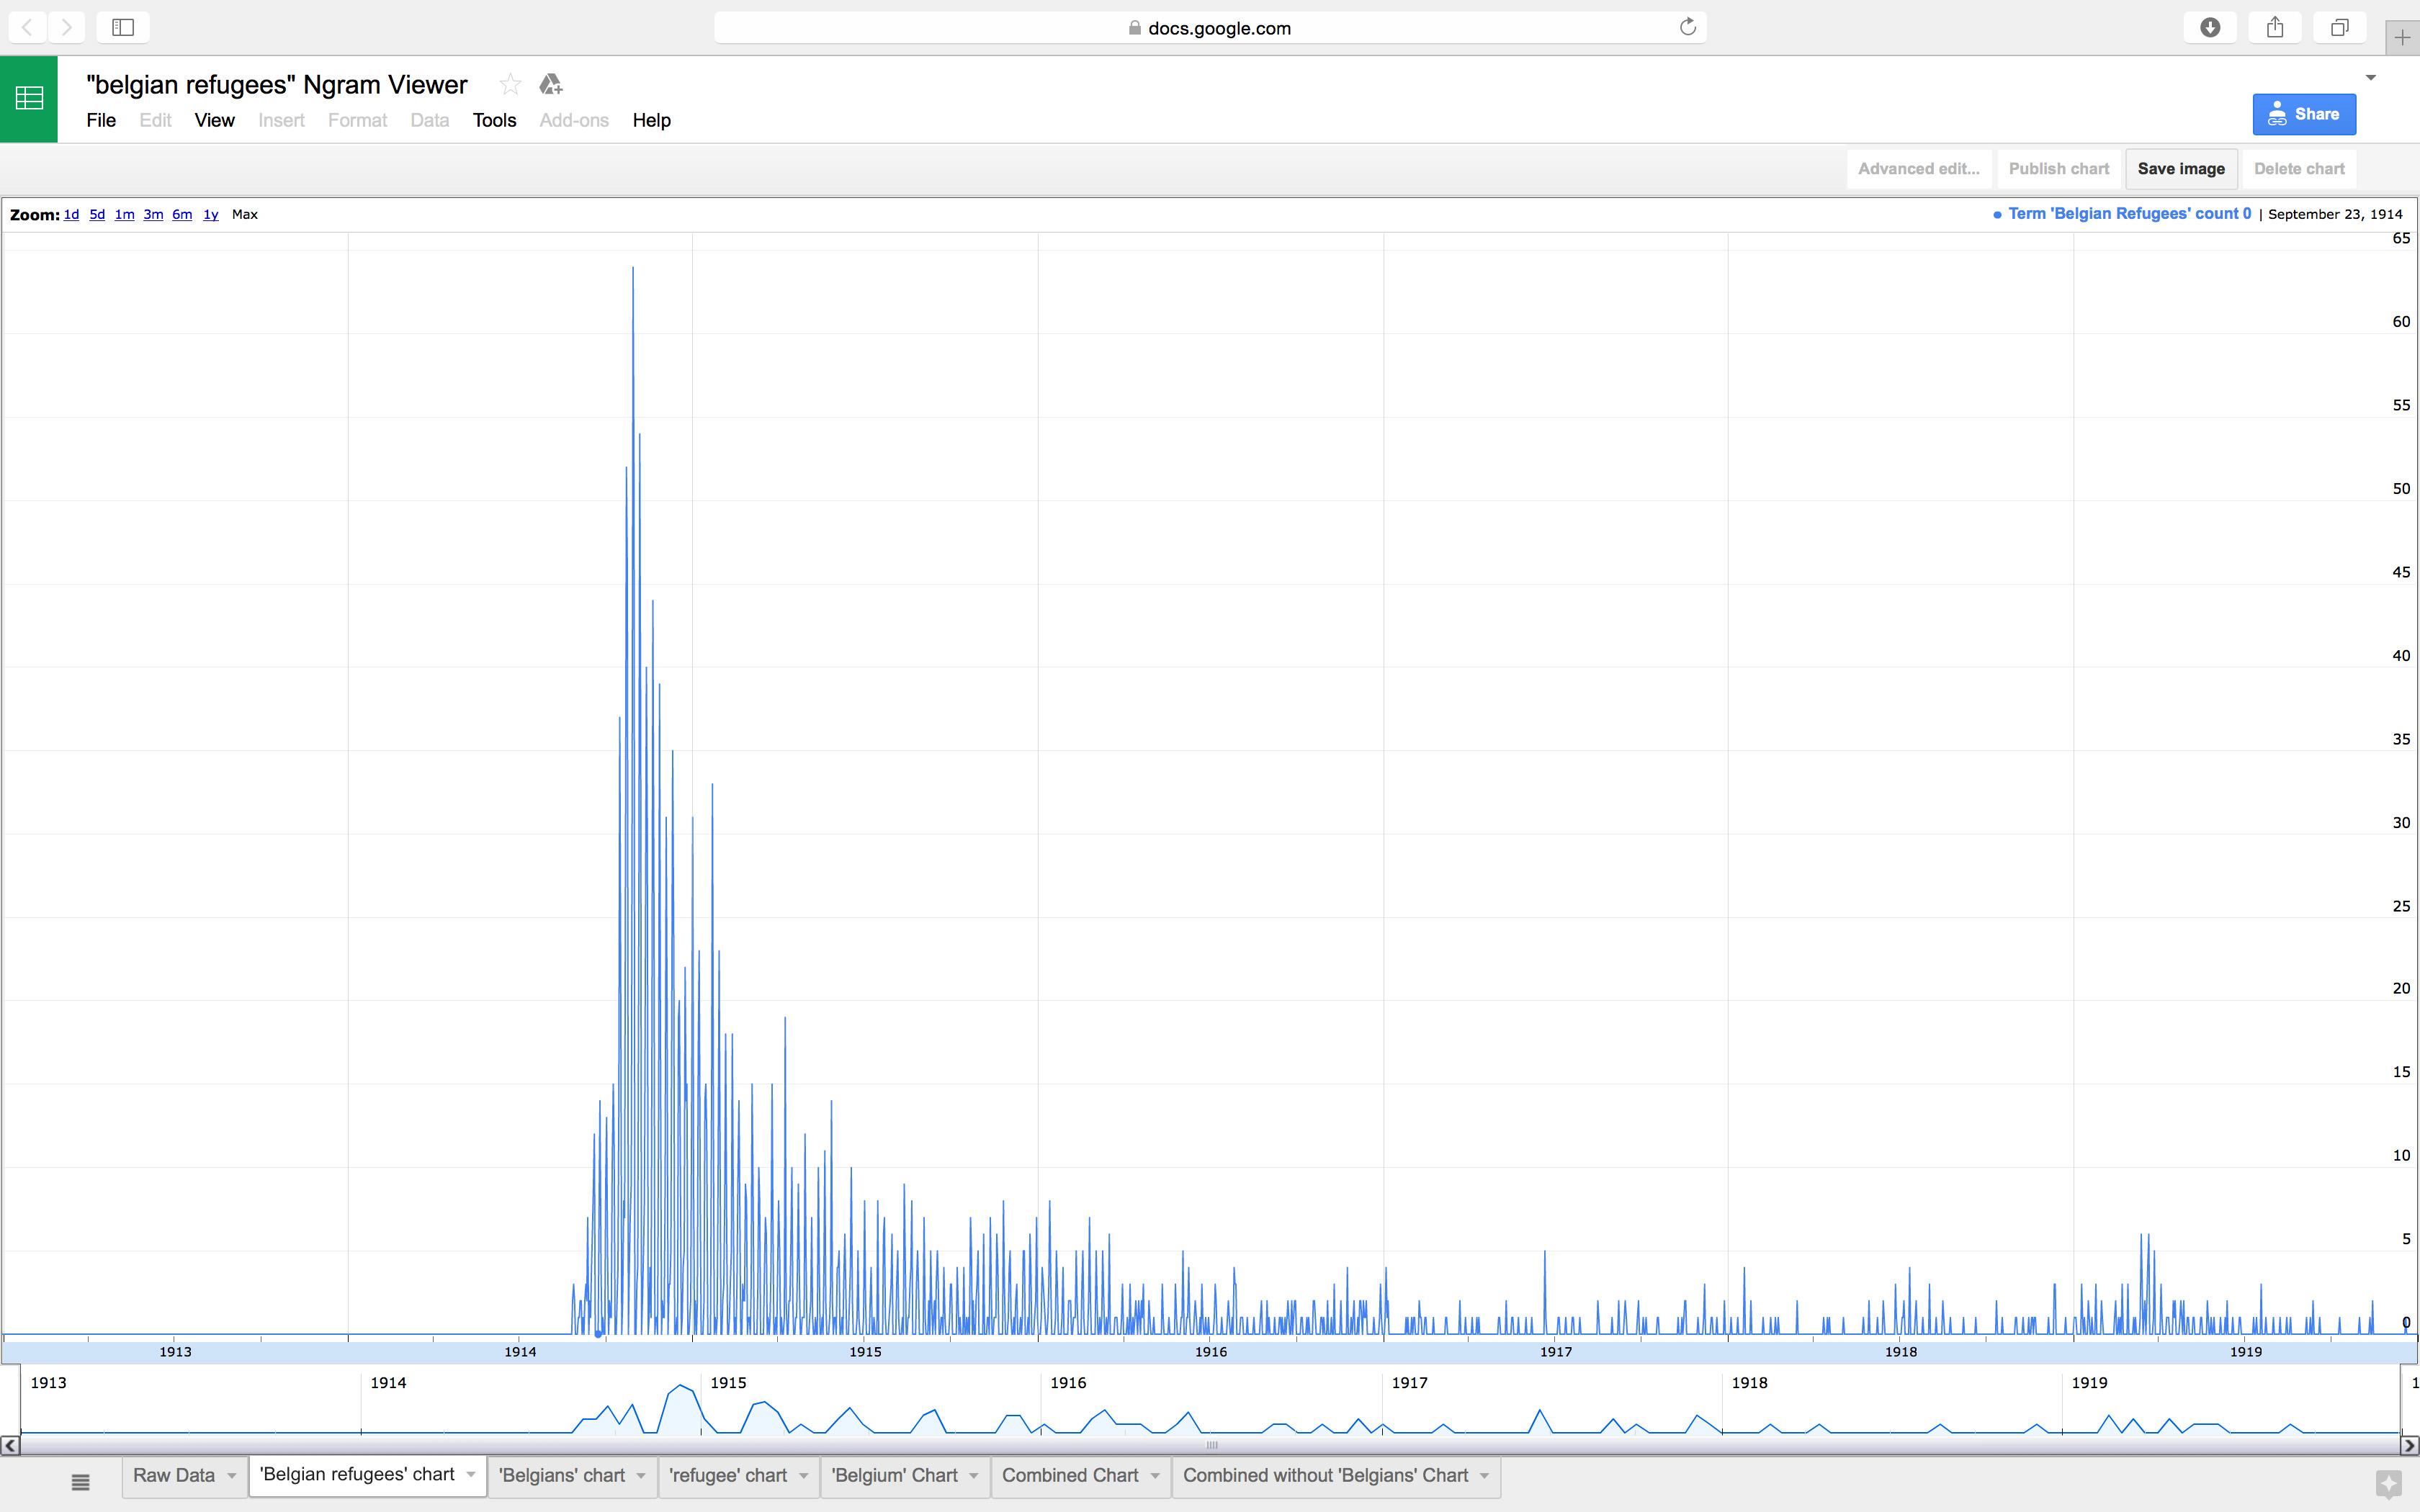
\includegraphics[scale=0.08]{img/fig2.jpg}
\caption{nGram of the term `Belgian refugees' in Welsh Newspapers Online}
\label{fig:2}
\end{figure}
%<Figure 2: nGram of the term ‘Belgian refugees’ in Welsh Newspapers Online>

\section{Creating better environments for drawing together multimedia content from a variety of sources for analysis and publication}

The attraction of working in a digital environment is the ability to integrate sources in a variety of formats, and to use them for new and unforeseen purposes. An example of working with hybrid, multimedia content can be seen in an AHRC funded project, \emph{The Snows of Yesteryear: Narrating Extreme Weather}\footnote{\url{Eira.llgc.org.uk}. The partners in the project were the Centre for Advanced Welsh and Celtic Studies at the University of Wales, the ACRE Project at the UK Met Office, the department of performance at Aberystwyth University, and Welsh performance artist, Eddie Ladd.}. The project was a creative collaboration to uncover archives in the collections of the National Library of Wales that contain information about the impact of extreme weather in Wales during the period from about 1700 (the pre-weather instrument period) to the 1960s. This included manuscripts (literary works, diaries, letters); printed materials, including Welsh ballads; and other material, including art works and manuscripts. These were digitized and made accessible to a team of climate scientists from the ACRE Project at the UK Met Office who used the data to fill gaps in the global picture of extreme weather in this period, and to use digital tools and methods to `map' and visualize incidents of extreme weather: floods, storms, freezing conditions, and incidents including the `year without a summer', in 1816 (after the Tambora volcano eruption caused severe climate abnormalities). The project also carried out community engagement, gathering interviews with local communities to share their experiences of extreme weather events within living memory: floods, storms, and snowfall. Form these two strands of evidence, we were able to construct two types of interpretation and analysis: the scientific visualisations; and also a public performance piece, \emph{Ghost Dance}, by Eddie Ladd: this drew on disparate narratives describing events of the winter of 1963 in an allegorical, not didactic way.

The project required sustaining a complex, hybrid archive of materials related to extreme weather impact in Wales, their analysis through performance and scientific visualization, and the communities that contribute this data. As such, it exemplifies the possibilities of digitally integrated research as set out in the Digital Humanities Manifesto: the ability to combine research, curation, and archive management to re-imagine the creation of digital content as a process of creative making, bringing together scholars and curators in ways that recast the role of each, driven by a shared goal of using historical sources for new purposes These approaches effect collaboration of disciplines and data types as an act of curation as much as a piece of scholarship, one in which scholars will not just create not just a collection of sources, but also effect a convergence of practices: artistic, scientific, and humanistic, and the ability to work with connected communities around the content\footnote{\url{http://manifesto.humanities.ucla.edu/}}. Documenting and publishing this sort of practice over the long term will also create a range of interesting issues -- how do we replicate the relationships between archives, scientific visualization, and performance? How is provenance of archives retained when embedded in a scientific visualization, or a performance? How will the convergence of digital and born digital be preserved and replicated over the long term? This form of knowledge production is an exciting means of determining the interface to information, data, and knowledge. It also raises significant information management research challenges associated with managing and sustaining complex collections over time, pushing the boundaries of what is currently known about stewardship and curation of humanities and cultural heritage content and data.

\bibliographystyle{sapauth-eng}
\bibliography{../../EAGLE}
\end{document}